\documentclass{article}

\usepackage{graphicx}
\usepackage{tikz}
\usepackage{tikzsymbols}
\usetikzlibrary{calc,patterns,shapes.geometric}
\pagestyle{empty}
\usepackage[margin=0pt]{geometry}
\geometry{papersize={14in,12in}}

\def\centerarc[#1](#2)(#3:#4:#5){\draw[#1] ($(#2)+({#5*cos(#3)},{#5*sin(#3)})$) arc (#3:#4:#5);}

\begin{document}
	\begin{figure}
		\centering
		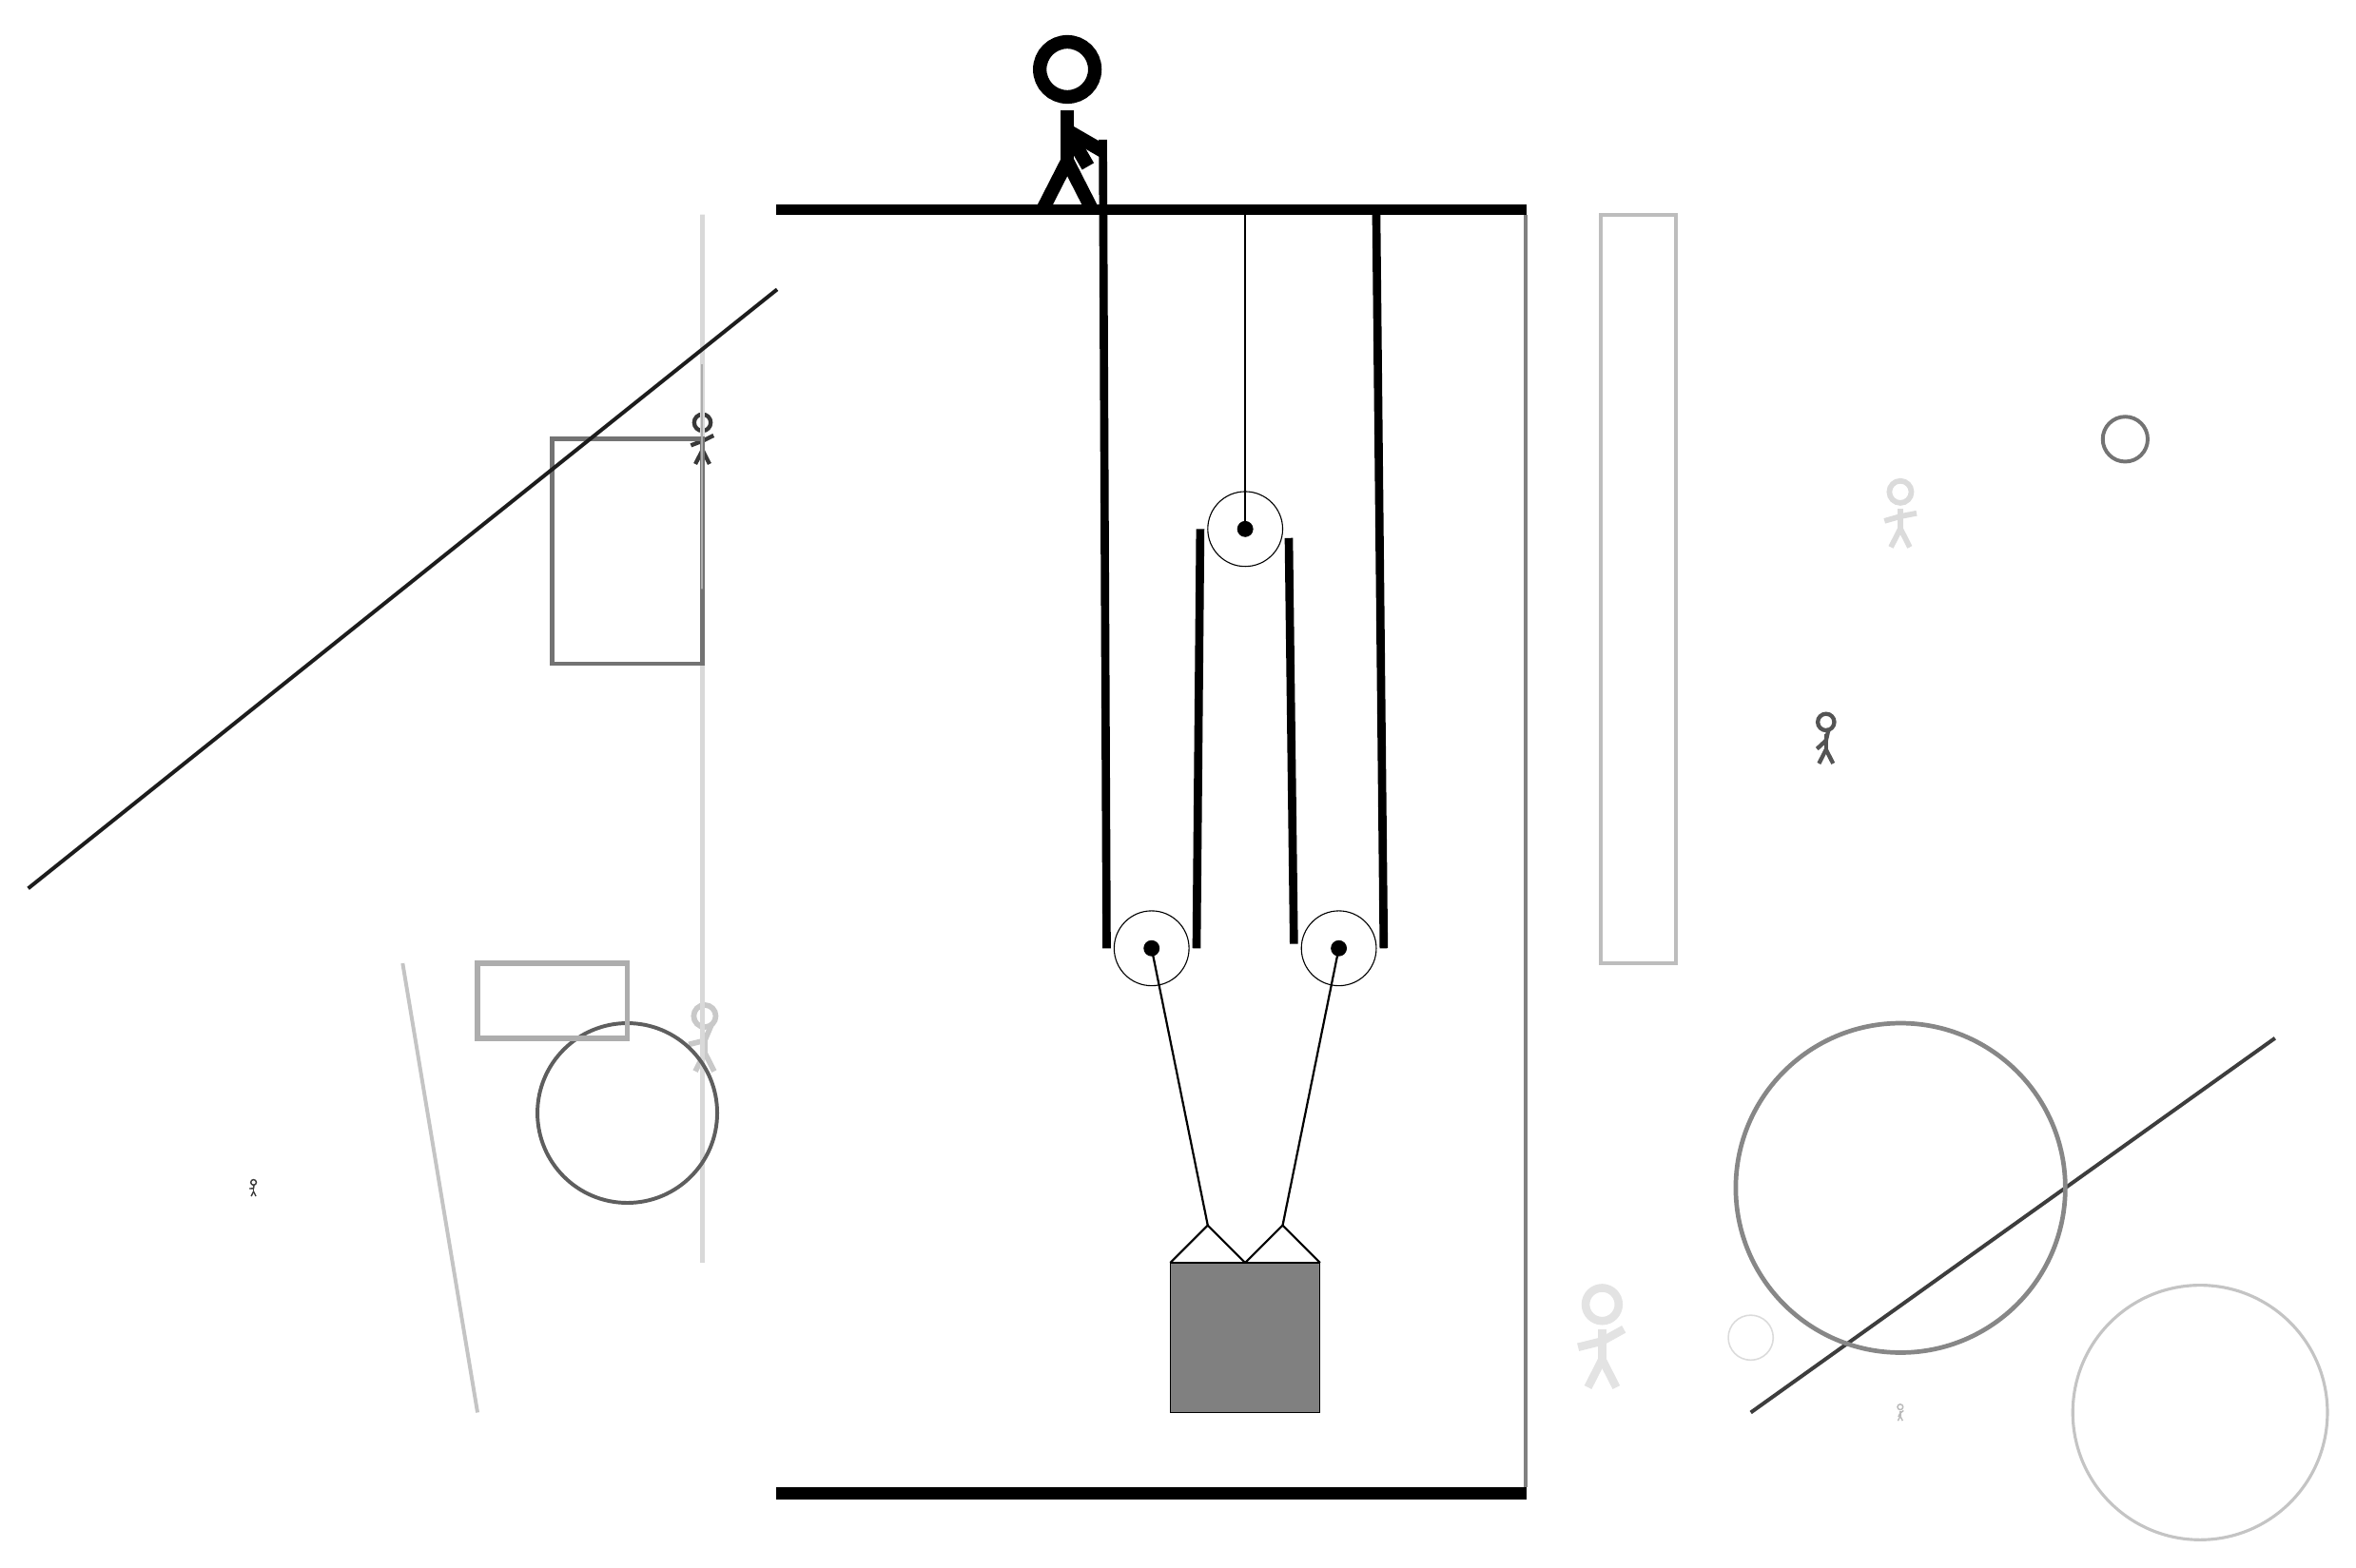
\begin{tikzpicture}
			%%%%% START %%%%%
			
			\draw[fill=black] (-4, 14) rectangle (6, 14.125);
			
			\draw (1, 4.2) circle (0.5);
			\draw[fill=black] (1, 4.2) circle (0.1);
			
			\draw (2.25, 9.8) circle (0.5);
			\draw[fill=black] (2.25, 9.8) circle (0.1);
			\draw[thick] (2.25, 9.8) -- (2.25, 14);
			
			\draw (3.5, 4.2) circle (0.5);
			\draw[fill=black] (3.5, 4.2) circle (0.1);
			
			\draw[thick] (3.5, 4.2) -- (2.75, 0.5);
			\draw[thick] (1, 4.2) -- (1.75, 0.5);
			\draw[thick]  (1.25, 0) -- (1.75, 0.5) -- (2.25, 0);
			\draw[thick]  (2.25, 0) -- (2.75, 0.5) -- (3.25, 0);
			\draw[fill=black!50] (1.25, 0) rectangle (3.25, -2);
			
			\draw[line width=1.1mm] (0.35, 15) --  (0.4, 4.2);
			\centerarc[line width=1.1mm](1, 4.2)(180:360:0.6);
			\draw[line width=1.1mm] (1.6, 4.2) -- (1.65, 9.8);
			\centerarc[line width=1.1mm](2.25, 9.8)(-20:180:0.6);
			\draw[line width=1.1mm](2.832, 9.68) -- (2.9, 4.26);
			\centerarc[line width=1.1mm](3.5, 4.2)(160:360:0.6);
			\draw[line width=1.1mm](4.1, 4.2) -- (4.0, 14);
			
			\node[line width=0.5mm, color=black!21] at (-5, 3) {\Strichmaxerl[4][14][67]};
			
			\node[line width=0.3mm, color=black!78] at (-5, 11) {\Strichmaxerl[3][21][26]};
			\node[line width=0.5mm, color=black!11] at (7, -1) {\Strichmaxerl[6][14][29]};
			\draw[line width=0.7mm, color=black!15] (-5, 0) rectangle (-5, 14);
			\draw[line width=0.6mm, color=black!55] (-5, 8) rectangle (-7, 11);
			\draw [line width=0.4mm, color=black!23](15, -2) circle (1.7);
			\node[line width=0.6mm, color=black!27] at (11, -2) {\Strichmaxerl[1][63][37]};
			\node[line width=0.5mm, color=black!67] at (10, 7) {\Strichmaxerl[3][43][77]};
			\draw[line width=0.5mm, color=black!76](9, -2) -- (16, 3);
			\draw [line width=0.5mm, color=black!55](14, 11) circle (0.3);
			
			\draw[line width=0.5mm, color=black!50](6, -3) -- (6, 14);
			\draw [line width=0.6mm, color=black!47](11, 1) circle (2.2);
			\node[line width=0.2mm, color=black!77] at (-11, 1) {\Strichmaxerl[1][2][83]};
			\draw[line width=0.5mm, color=black!89](-4, 13) -- (-14, 5);
			\draw [line width=0.5mm, color=black!63](-6, 2) circle (1.2);
			\draw [line width=0.2mm, color=black!14](9, -1) circle (0.3);
			
			\draw[line width=0.3mm, color=black!32] (-5, 12) rectangle (-5, 9);
			\node[line width=0.6mm, color=black!14] at (11, 10) {\Strichmaxerl[4][16][11]};
			\draw[line width=0.5mm, color=black!23](-8, -2) -- (-9, 4);
			\draw[line width=0.7mm, color=black!32] (-6, 4) rectangle (-8, 3);
			\draw[line width=0.5mm, color=black!26] (7, 14) rectangle (8, 4);
			
			\node at (-0.07, 15.2) {\Strichmaxerl[10][120][-30]};
			
			\draw[fill=black] (-4, -3) rectangle (6, -3.15);
			
			%%%%% END %%%%%
		\end{tikzpicture}
	\end{figure}	
\end{document}